\chapter{Tests}

\section{Schematics}

float barrier command to ensure that text stays close to the picture but no text from after the picture.

\subsection{part 1}

\begin{figure}[ht]
    \centering
    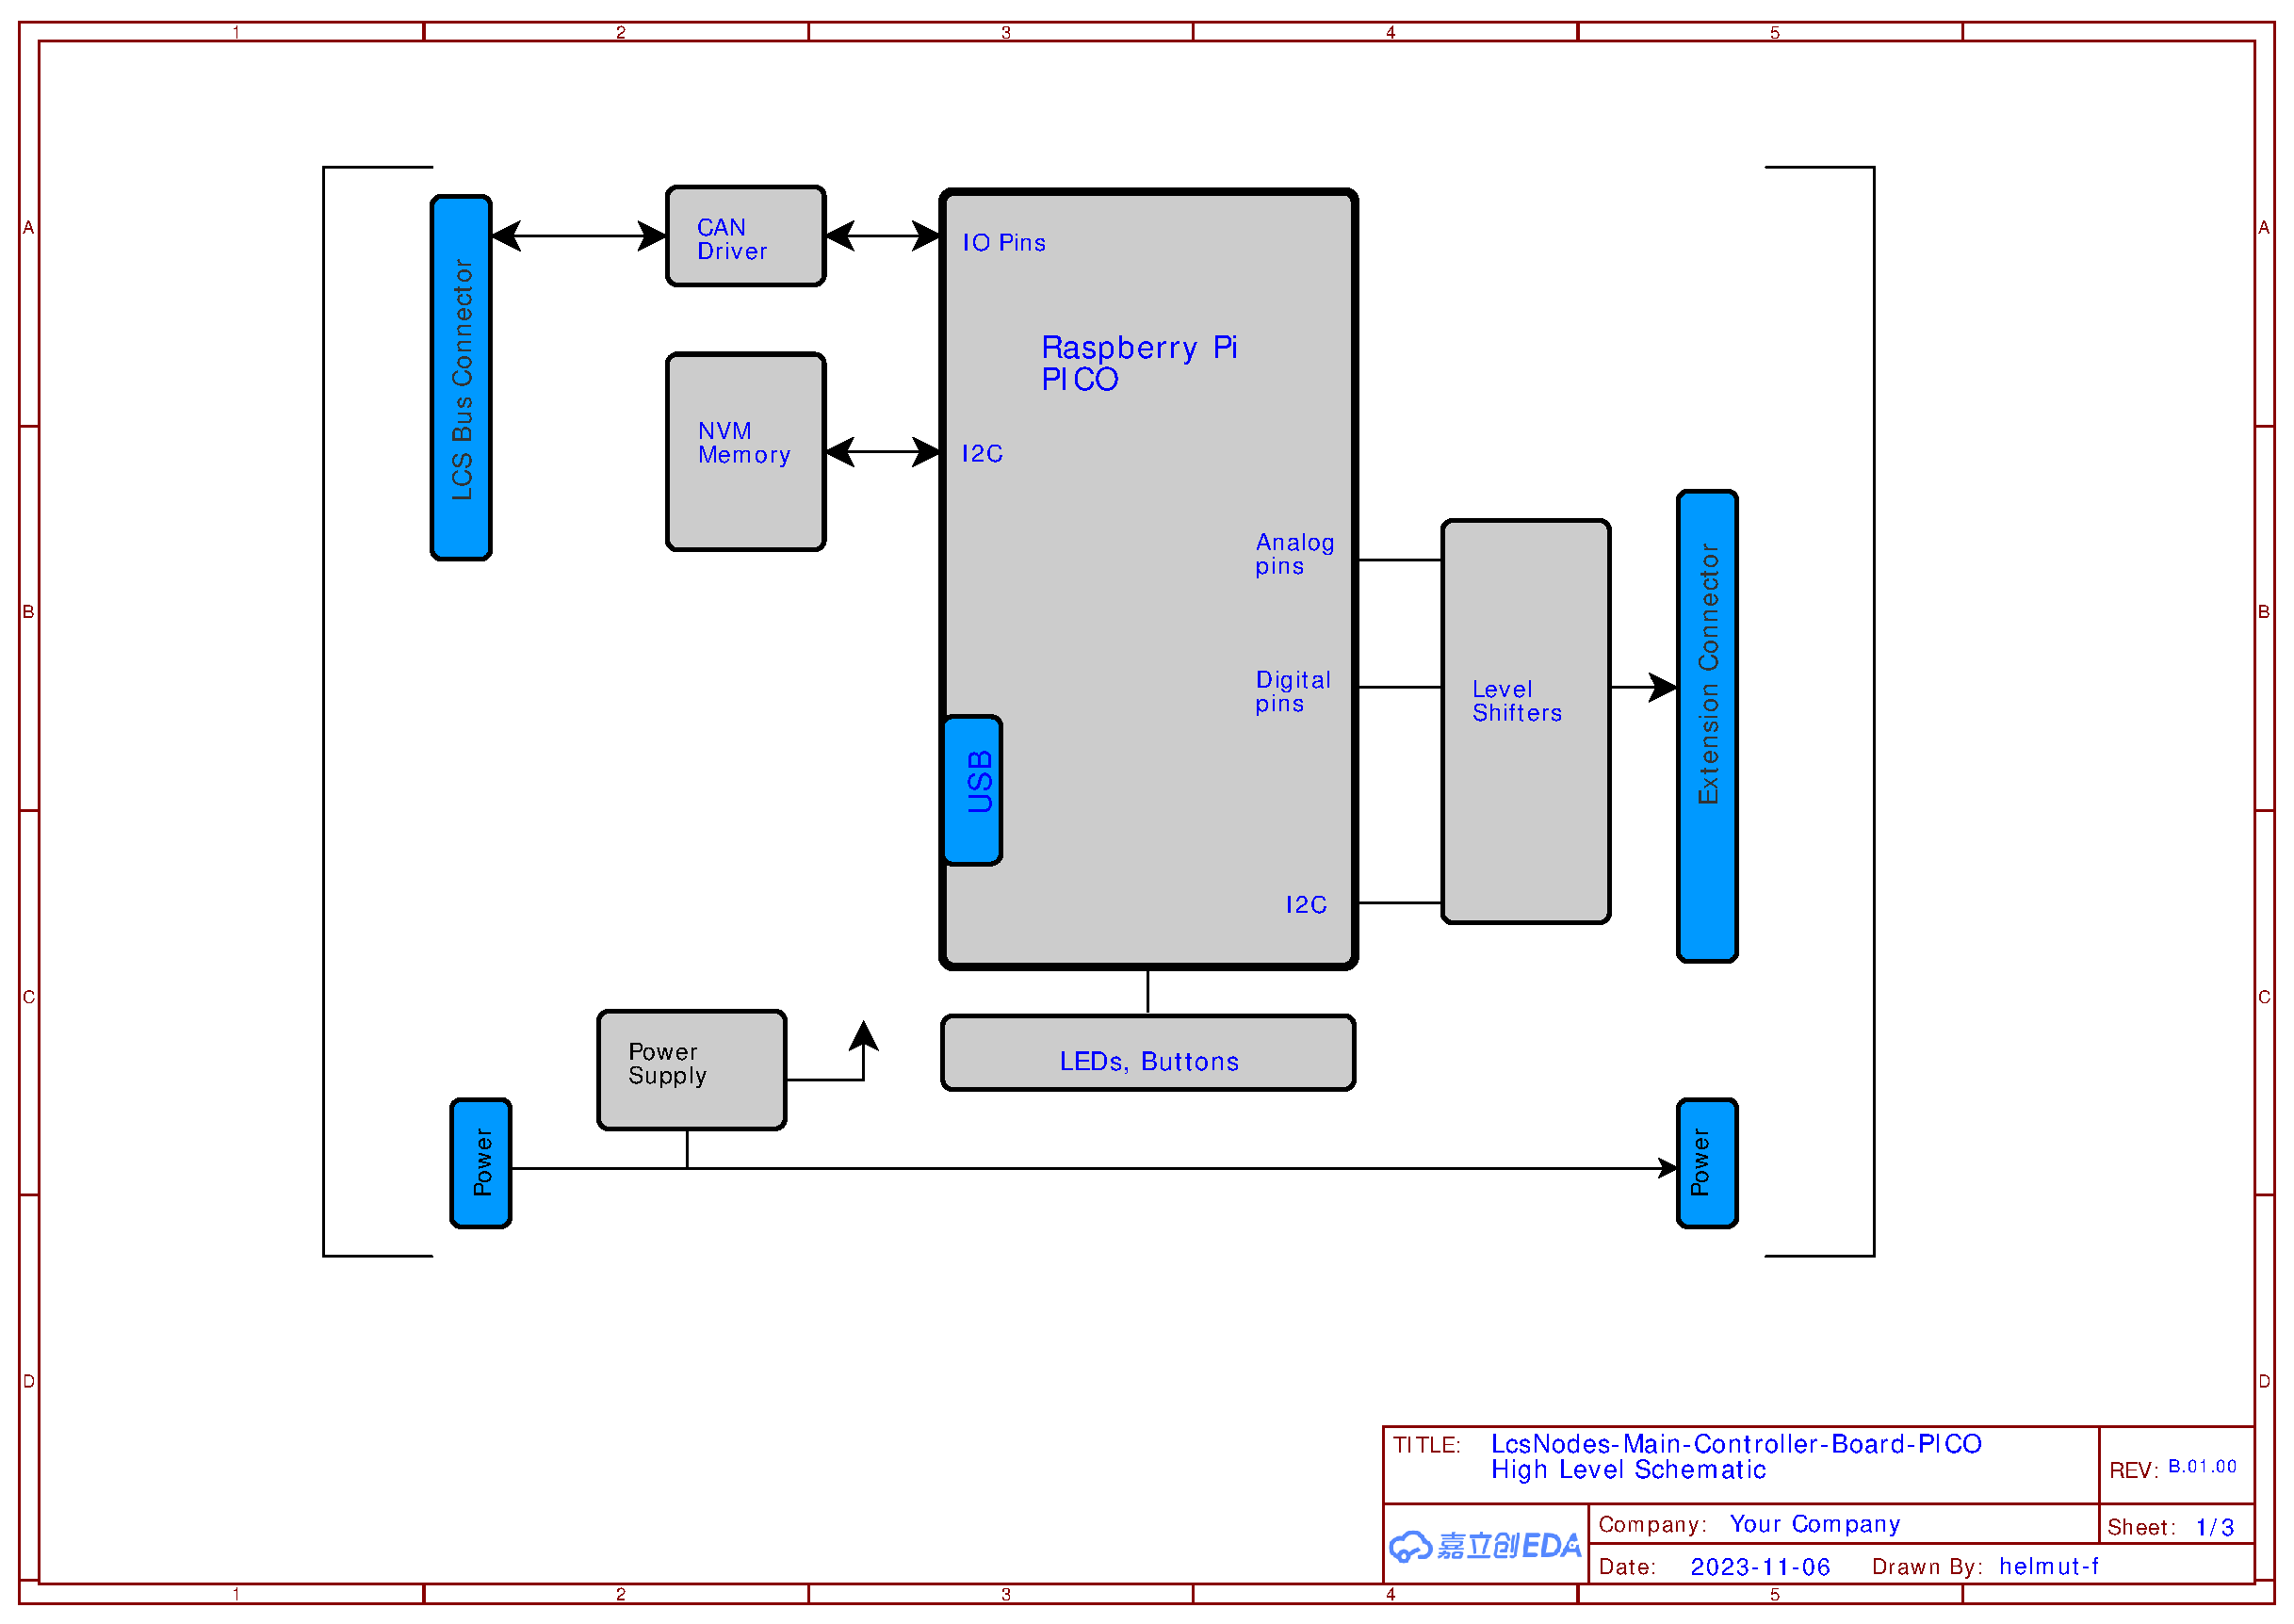
\includegraphics[page=1, width=\textwidth]{./schematics/Schematic_LcsNodes-Main-Controller-Board.pdf}
\end{figure}

\FloatBarrier

\subsection{part 2}
\begin{figure}[ht]
    \centering
    \includegraphics[page=2, width=\textwidth]{./schematics/Schematic_LcsNodes-Main-Controller-Board.pdf}
\end{figure}

\FloatBarrier

\subsection{part 3}
\begin{figure}[ht]
    \centering
    \includegraphics[page=3, width=\textwidth]{./schematics/Schematic_LcsNodes-Main-Controller-Board.pdf}
\end{figure}

\FloatBarrier


\section{Lists}

\subsection{A simple list}

\begin{itemize}
    \item First bullet point
    \item Second bullet point
    \item Third bullet point
\end{itemize}



\subsection{An instruction word layout}

A little test for an instruction word layout ... will be a bit fiddling work ... 

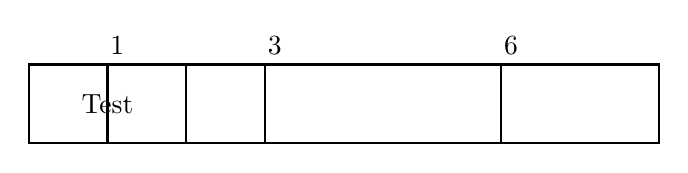
\begin{tikzpicture}
    \draw[thick] (0, 0) rectangle (8, 1); % Simple rectangle
    \node at (1, 0.5) {Test};   % Centered text
    \draw[thick] (2, 0) -- (2, 1);

    \foreach \x in {1, 3, 6} {
        \draw[thick] (\x, 0) -- (\x, 1); % Vertical line
        \node[above] at (\x + 0.125, 1) {\x}; % a number above the field
    }

\end{tikzpicture}


First attempt ...

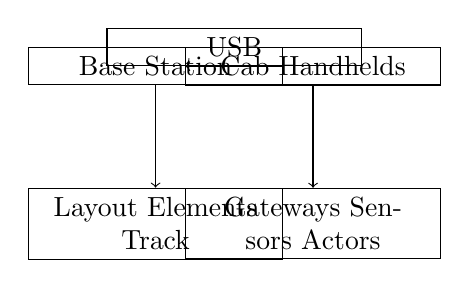
\begin{tikzpicture}[node distance=2cm, every node/.style={draw, text width=3cm, align=center}]
% Nodes
\node (base) {Base Station};
\node[right of=base] (cab) {Cab Handhelds};
\node[below of=cab] (gateways) {Gateways Sensors Actors};
\node[below of=base] (track) {Layout Elements \\ Track};

% Arrows
\draw[->] (base) -- (cab) node[midway, above] {USB};
\draw[->] (cab) -- (gateways);
\draw[->] (base) -- (track);

\end{tikzpicture}